\documentclass[]{article}
\usepackage{lmodern}
\usepackage{amssymb,amsmath}
\usepackage{ifxetex,ifluatex}
\usepackage{fixltx2e} % provides \textsubscript
\ifnum 0\ifxetex 1\fi\ifluatex 1\fi=0 % if pdftex
  \usepackage[T1]{fontenc}
  \usepackage[utf8]{inputenc}
\else % if luatex or xelatex
  \ifxetex
    \usepackage{mathspec}
  \else
    \usepackage{fontspec}
  \fi
  \defaultfontfeatures{Ligatures=TeX,Scale=MatchLowercase}
\fi
% use upquote if available, for straight quotes in verbatim environments
\IfFileExists{upquote.sty}{\usepackage{upquote}}{}
% use microtype if available
\IfFileExists{microtype.sty}{%
\usepackage{microtype}
\UseMicrotypeSet[protrusion]{basicmath} % disable protrusion for tt fonts
}{}
\usepackage[margin=1in]{geometry}
\usepackage{hyperref}
\hypersetup{unicode=true,
            pdftitle={Harvard Data Science Capstone},
            pdfauthor={Tyson Klein},
            pdfborder={0 0 0},
            breaklinks=true}
\urlstyle{same}  % don't use monospace font for urls
\usepackage{longtable,booktabs}
\usepackage{graphicx,grffile}
\makeatletter
\def\maxwidth{\ifdim\Gin@nat@width>\linewidth\linewidth\else\Gin@nat@width\fi}
\def\maxheight{\ifdim\Gin@nat@height>\textheight\textheight\else\Gin@nat@height\fi}
\makeatother
% Scale images if necessary, so that they will not overflow the page
% margins by default, and it is still possible to overwrite the defaults
% using explicit options in \includegraphics[width, height, ...]{}
\setkeys{Gin}{width=\maxwidth,height=\maxheight,keepaspectratio}
\IfFileExists{parskip.sty}{%
\usepackage{parskip}
}{% else
\setlength{\parindent}{0pt}
\setlength{\parskip}{6pt plus 2pt minus 1pt}
}
\setlength{\emergencystretch}{3em}  % prevent overfull lines
\providecommand{\tightlist}{%
  \setlength{\itemsep}{0pt}\setlength{\parskip}{0pt}}
\setcounter{secnumdepth}{0}
% Redefines (sub)paragraphs to behave more like sections
\ifx\paragraph\undefined\else
\let\oldparagraph\paragraph
\renewcommand{\paragraph}[1]{\oldparagraph{#1}\mbox{}}
\fi
\ifx\subparagraph\undefined\else
\let\oldsubparagraph\subparagraph
\renewcommand{\subparagraph}[1]{\oldsubparagraph{#1}\mbox{}}
\fi

%%% Use protect on footnotes to avoid problems with footnotes in titles
\let\rmarkdownfootnote\footnote%
\def\footnote{\protect\rmarkdownfootnote}

%%% Change title format to be more compact
\usepackage{titling}

% Create subtitle command for use in maketitle
\newcommand{\subtitle}[1]{
  \posttitle{
    \begin{center}\large#1\end{center}
    }
}

\setlength{\droptitle}{-2em}

  \title{Harvard Data Science Capstone}
    \pretitle{\vspace{\droptitle}\centering\huge}
  \posttitle{\par}
    \author{Tyson Klein}
    \preauthor{\centering\large\emph}
  \postauthor{\par}
      \predate{\centering\large\emph}
  \postdate{\par}
    \date{October 22, 2018}


\begin{document}
\maketitle

\section{Analysis of RedBubble.com sales by
TysonK}\label{analysis-of-redbubble.com-sales-by-tysonk}

\subsection{Running this Analysis}\label{running-this-analysis}

To recreate this analysis at home, you can clone this repo and open this
project in Rstudio, then run the R scripts in the following order:
package-installer.r -\textgreater{} wrangle-data.r -\textgreater{}
distribution-analysis.r -\textgreater{} generate-plots.r -\textgreater{}
then Knit Readme.Rmd

\subsection{An Introdution}\label{an-introdution}

RedBubble is one of the longest running and diverse Print-On-Demand
(POD) art websites in the world, offering artists everywhere the
opportunity to make money by selling their works on a range of products
without having to get involved with any of the logistics.

RedBubble, like many of its contemporaries, has a `passive' approach for
the artist. You upload your designs as images and they do everything
else. This means that all sales made are pure profit on the artists
side.

About a year and a half ago I opened
\href{https://www.redbubble.com/people/tysonk?ref=account-nav-dropdown\&asc=u}{my
Redbubble store}. The specifics of my store aren't entirely important to
this report, but there are some important details that will emerge again
later. Most designs in my store have something to do with National Parks
from English speaking countries around the world, and the remainder of
the designs are an eclectic mix of outdoors-themed and quirky products
meant to appeal to a general audience.

My store began to gain traction and some interesting patterns began to
emerge. For example, although RedBubble offers designs to be printed on
products ranging from coffee mugs to T shirts to throw pillows, by far
my most successful item was the sticker.

To date, stickers account for 98.5\% of all items sold and 96.2\% of all
profit.

\subsection{Daily Users and Profit}\label{daily-users-and-profit}

Below is the profit per day of my store since May 1st, 2017, measured in
Canadian Dollars(red), and the same graph instead measuring unique daily
users (turquoise).

\begin{center}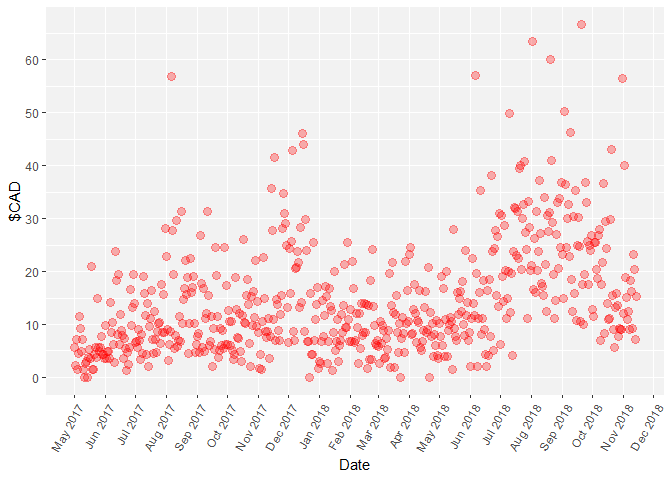
\includegraphics{Readme_files/figure-latex/daily sales and user plot-1} \end{center}

\begin{center}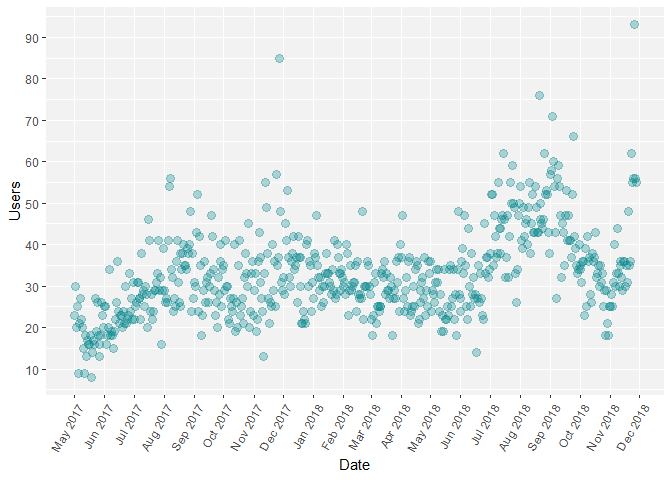
\includegraphics{Readme_files/figure-latex/daily sales and user plot-2} \end{center}

Clearly a trend exists with both data sets. First, there are some
noticeable peaks and valleys that seem to line up with both. These
represent busy and slow periods for the store, but before we can better
quantify \emph{how} busy or slow, this data must be better understood
and manipulated.

\subsection{Rolling average and distribution
fitting}\label{rolling-average-and-distribution-fitting}

To begin, a useful tool to analyze the overall trend of an extended
period for such a random data set is a \textbf{rolling average}. This is
an alpha adjusted average where \emph{average.today = actual.yesterday*A
+ average.yesterday*(1 - A)}. Calculating the average for day \textbf{N}
uses only data from day \textbf{N - 1} and earlier. This is done to
prevent the average from being over-informed when constructing
confidence intervals.

A has to be appropriately small so that the rolling average isn't
completely changed for every outlier day, yet large enough to respond
quickly to the profit trend. All proceeding A's are set at 0.07.

Now that we have an average to compare every day to, another valuable
statistic to learn is the day-to-day variation in both data sets. For
brevity, this analysis will only be done on the daily users, but the
process is identical.

A great way to do this is to fit our varied data to a series of
plausible distributions and observe which distribution best represents
the variance. Unfortunately, these data sets exhibit trends which
prevent us from simply measuring the variance between \emph{all} data
points. This is a perfect use for our computed rolling average, and
instead of simply measuring the variance between daily users, we can
account for the trend by dividing each daily user data point by its
corresponding user rolling average. This can be thought of as
\textbf{Adjusting} our data set to account for time-dependent trends,
preserving the variance and yielding the following:

\begin{center}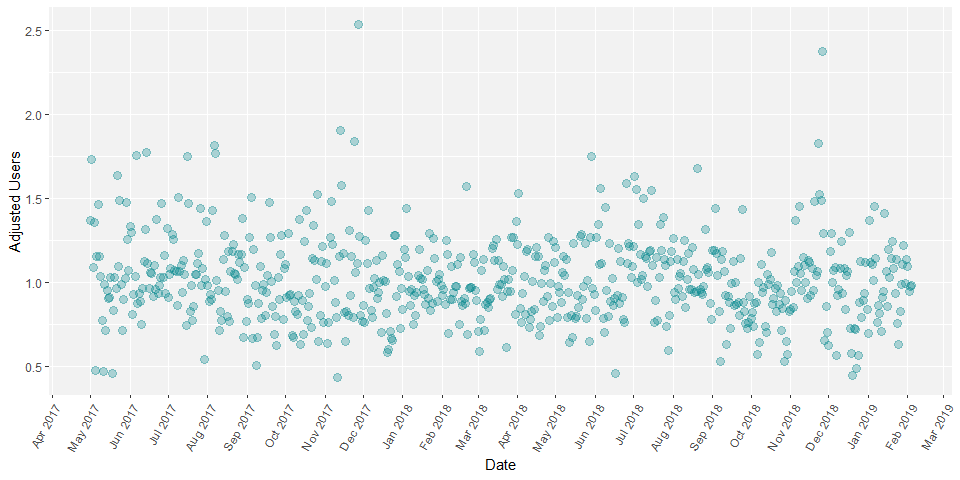
\includegraphics{Readme_files/figure-latex/adjusted daily users plot-1} \end{center}

These points represent how each day relates to the rolling average. Five
distributions were used to fit this data; Normal, Gamma, Weibull, Dagum,
and GEV (Generalized Extreme Value). These five were chosen specifically
because they are some of the most common distributions for inter-arrival
times (With exception to the Normal distribution, which is included for
comparison purposes), and random variables like daily profit and unique
users can be thought of the same way, since there is a hard minimum (0),
which is very unlikely, and practically infinite maximum.

\begin{center}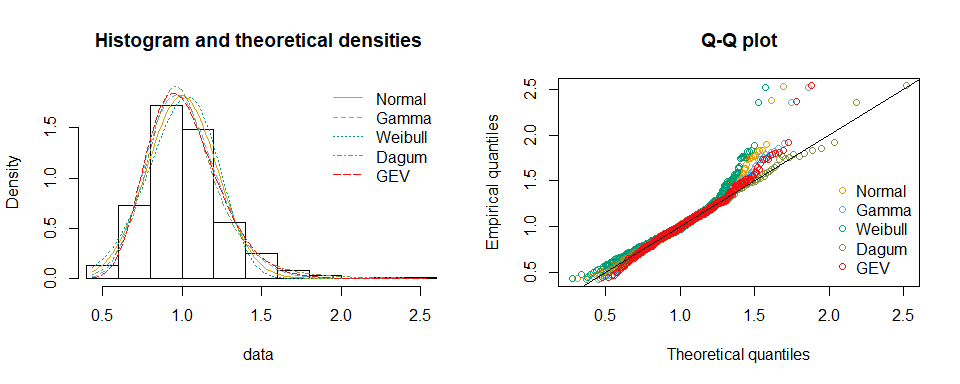
\includegraphics{Readme_files/figure-latex/User distribution fits-1} \end{center}

As you can see from these plots, these functions all look very similar,
although the Q-Q plot points to the Dagum function being the best fit. A
better way to cut through the subjectivity of selecting a distribution
is summarizing with the Kolmogorov-Smirnov fitness test. Below is a
table with results for all five distributions.

\begin{longtable}[]{@{}lrr@{}}
\toprule
Distribution & Test.Statistic & P.value\tabularnewline
\midrule
\endhead
Normal & 0.0395 & 0.2231\tabularnewline
Gamma & 0.0231 & 0.8468\tabularnewline
Weibull & 0.0519 & 0.0457\tabularnewline
Dagum & 0.0157 & 0.9952\tabularnewline
GEV & 0.0276 & 0.6573\tabularnewline
\bottomrule
\end{longtable}

While the KS test only eliminated the Weibull distribution on a p
\textless{} 0.05 threshold, we can see that the KS test also supports
our theory that the data fits a Dagum distribution very well.

\subsection{Naive Trend Analysis}\label{naive-trend-analysis}

Below are the original sales and user charts, now with the rolling
average (dark line) and 90\% confidence intervals (light lines)
constructed from the Dagum distribution. This confidence interval
represents where 90\% of all data points will exist between. This is the
first opportunity to see the story being told by the data. If you pay
close attention to the dates of some of the peaks and valleys, there are
four clear trends.

\begin{enumerate}
\def\labelenumi{\arabic{enumi}.}
\tightlist
\item
  Both tend to be higher during the late summer months.
\item
  Both tend to be higher during mid-November to mid-December.
\item
  Both, in general, increase over time.
\item
  There is less variance in daily users than daily sales.
\end{enumerate}

\begin{center}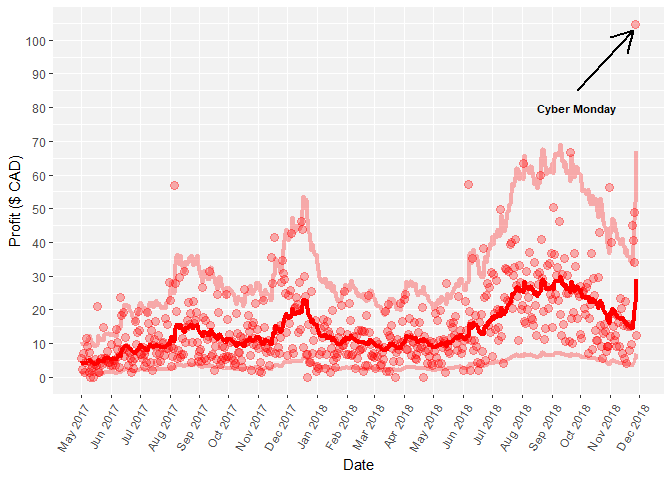
\includegraphics{Readme_files/figure-latex/daily sales and user plot with rolling average and CI-1} \end{center}

\begin{center}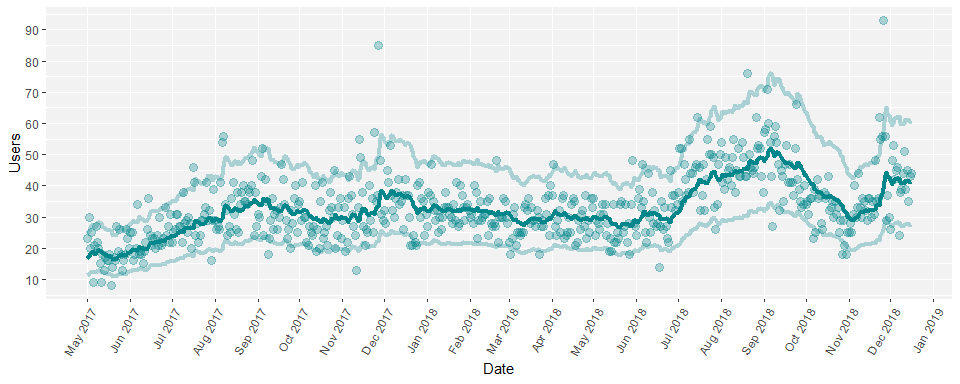
\includegraphics{Readme_files/figure-latex/daily sales and user plot with rolling average and CI-2} \end{center}

\subsection{Factors to Consider}\label{factors-to-consider}

A very important thing to understand about a RedBubble store is that
unique users have a direct relationship with daily sales. There are a
few steps involved to get from one to the other, and the easiest way to
illustrate this path is to consider an average customer.

Let's say Jim has decided he wants to buy a sticker for
\href{https://www.redbubble.com/people/tysonk/works/33710123-banff-national-park-basic?asc=u\&p=sticker}{Banff
National Park} after a recent holiday. Jim finds the RedBubble
storefront for my sticker, and the first stop on the path occurs.
\textbf{Jim decides if he wants to buy this product}. This interaction,
which I call the \emph{should I?} factor, is a random variable with
possible outcomes of \emph{yes} or \emph{no}.

Assuming Jim loves the design and chooses to buy it, he adds it to his
cart. Jim now has another important decision to make; \textbf{Jim
decides if he wants to buy another product}. Almost always the answer to
this is no, but again this interaction introduces another factor I call
\emph{how many?}. This is also a random variable with possible outcomes
\emph{1} to \emph{infinite}, heavily weighted towards 1.

Now that Jim has, say, a sticker and a T-shirt in his cart, he checks
out to complete his order. There is one more important random variable
to consider, and that is summarized by \textbf{How much profit does each
product produce?}. This is a very important factor, and one of the
variables that the artist has the most control over, called \emph{what
cost?}. It completely depends on the product, sale, and set margin for
the artist but can range from \emph{0} to \emph{infinite}, weighted
towards an average value dictated by the most commonly sold item.

The sale is now complete. Jim, the \textbf{user}, has completed an
\textbf{order} with the sticker and T-shirt representing multiple
\textbf{units}, for some \textbf{profit}. This directional flow of
actions results in much more variance on the profit end compared to the
user end and explains \#4 on our list of noticed trends.

\subsection{Analysis of Factors}\label{analysis-of-factors}

\subsubsection{Exposure}\label{exposure}

The success of this store, or really any merchandise business, resides
in how and what we change to influence these factors. To start, we can
look at the implied first factor: \emph{exposure}. This is where I would
have an absolute hay-day if I were privy to the data RedBubble collects
internally. Before we can influence a customer interaction, they must
see the webpage.

Unfortunately for the artists, there is very little that can be done to
increase exposure. RedBubble is a wild-west implementation of the POD
model: everyone uploads whatever they want, and the cream rises to the
top. One could argue that this is the best possible implementation,
where the best designs get rewarded the most, but that doesn't
necessarily happen.

RedBubble designs get more ad-targets and raise higher in internal
search rankings based on their sales record. What does this mean? A
mediocre design that has been on the store for a while with modest sales
numbers can be on the first page of search results whereas a great
design that was recently uploaded with hardly any sales will be buried
in the later pages of a search result.

If I was a betting man (a great stance for an aspiring analyst), I would
say that search rank has a hell of a lot more to do with the success of
a single design than the quality of that design. What ends up happening
with this meritocratic approach is that page 1 designs stay on page 1
entirely because they sell better than page 2+ designs. Many times, I
have uploaded a design only to sell a grand total of 0 products within
the fist several months of its existence. Then, if a I get lucky and a
\textbf{single} person buys this design, it shoots up in the search
rankings past all the other un-bought designs. Suddenly, that design
turns into a hit.

To gain some autonomy over this seemingly unfair beginning of a design
life-cycle, I batch uploaded a series of designs, \textbf{bought them
all} with my second account, and spent the next few months making sales
of all of these designs having been kick started higher in the search
rankings.

For the average design in my store, the sales have slowly improved over
time as each individual ranking creeps closer and closer to its rightful
place in the search results. Often that happens to be on page 1, but
after some time the search ranking stabilizes. I believe this is one of
the main influences of \#3 of the noticed trends: Both users and Sales,
in general, increase over time.

\subsubsection{Should I?}\label{should-i}

Assuming the exposure of our design leads a user to click on it, the
next factor to consider is \emph{should I?}. As mentioned before, this
is a random variable with possible outcomes \emph{yes} or \emph{no}.
These can instead be thought of as \emph{1} or \emph{0}, with an
expected value somewhere in between. This value represents the
\textbf{probability of a user making a purchase} and is easily
represented as the \emph{average daily orders / average daily users}.

\begin{center}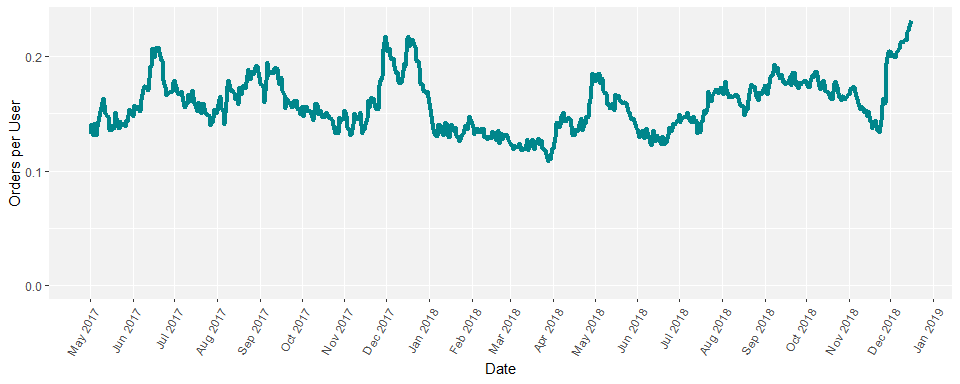
\includegraphics{Readme_files/figure-latex/daily Order per user plot-1} \end{center}

This graph seems to be fairly stable and doesn't change in response to
developments in my store and added designs. Instead, there are two
possible theories I have for the trend.

\begin{enumerate}
\def\labelenumi{\arabic{enumi}.}
\item
  The value is higher based on the quality of the design. This is
  approximately constant for my store because my set of designs are all
  very similar and most have existed since the start date of May 1st,
  2017. I would imaging talented designers would have this value higher
  than the \textasciitilde{}20\% purchase rate that I am showing.
\item
  The values fluctuate based on buyer desperation. I think it is no
  coincidence that the highest peak on this graph occurs in the month
  leading up to Christmas. Buyers are looking for gifts for loved ones
  and are more likely to make a purchase because they either aren't as
  scrutinous when they aren't buying for themselves or feel pressured
  from the in-site sales advertisements all over the webpage at that
  time of year. The dip in desperation after the holidays may also point
  to a lack of available spending money for customers.
\end{enumerate}

\subsubsection{How Many?}\label{how-many}

As mentioned before, most orders contain only a single unit. Below is a
histogram of Units per Order.

\begin{center}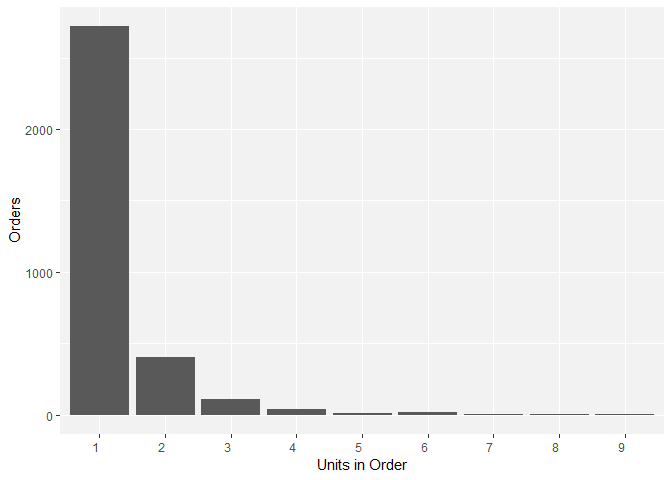
\includegraphics{Readme_files/figure-latex/units per order hist-1} \end{center}

This isn't necessarily because users usually only buy a single item; in
fact, it is usually the opposite. RedBubble has cleverly made their
products available at scale-able deals, discounting your whole order of
stickers based on how many you decide to purchase.

Barring differences in the exchange rate between USD and CAD, an average
full price sticker sold in the United States nets about \$4.05 in
profit. This is quantified in a histogram of US sticker sales by profit
per sticker.

\begin{center}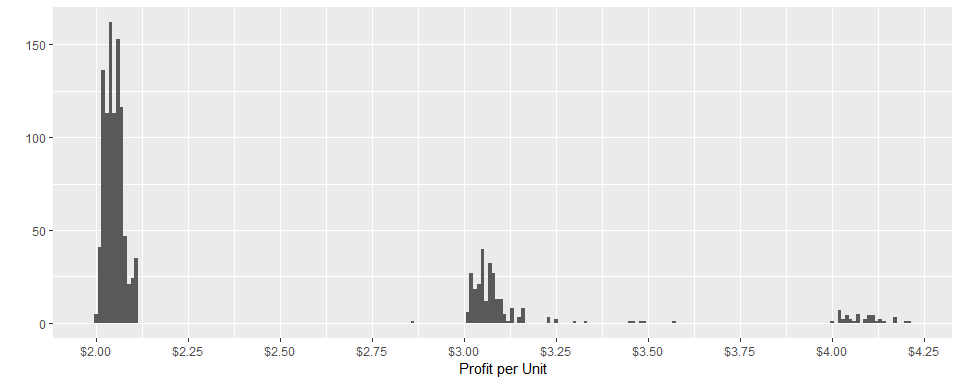
\includegraphics{Readme_files/figure-latex/unit profit hist-1} \end{center}

The small bump on the right side of this graph at just over \$4.00
represents these full price purchases, but you may have noticed that it
is by no means the largest bump on this graph. The two other bumps are
both very closely packed together, and clearly show that something else
is going on. Below is the same graph with lines representing various
levels of discount from full price.

\begin{center}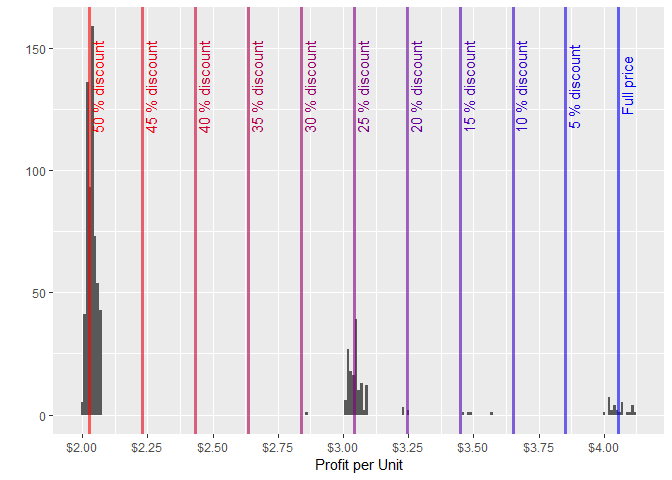
\includegraphics{Readme_files/figure-latex/unit profit hist with discount-1} \end{center}

This illustrates the discount strategy RedBubble is using. When you have
one sticker in your cart, a popup will notify you before checking out
that you can save 25\% if you buy 5 or more stickers and 50\% if you buy
10 or more stickers. Since there is no other way to buy a sticker from
my store at less than the full profit margin of \textasciitilde{}\$4.05
(other than short seasonal discounts of 15\%, 20\% and 30\% shown with
the tiny bumps on the graph), these two bumps represent people taking
advantage of these discounts. 76.8\% of all stickers are bought with the
10+ stickers for 50\% off discount, 19.5\% are bought with the 5+
stickers for 25\% off discount, and only 3.7\% of stickers are purchased
at full price.

Why then are most of my orders just single stickers? The benefit of
having such a huge open marketplace is that users have a ton of designs
to choose from. This means that orders of 10+ stickers will very rarely
have 2 designs by the same designer. The only reason people buy more
than one of my designs in a single order is because most of my designs
are in related series (for example, someone buys a Jasper and Banff
sticker because they have been to both).

Unfortunately, just like exposure, there is very little that can be done
to influence this factor. The only possible thing I have control over
for this \emph{how many?} factor is to make various series of related
designs on my store, and making related designs navigable to each other
via RedBubble's Collection feature.

\subsection{Coming Soon}\label{coming-soon}


\end{document}
